\documentclass[tikz,border=7pt]{standalone}
\usepackage{amsmath}
\usetikzlibrary{positioning,arrows.meta,fit}

\tikzset{
  comp/.style={draw,rectangle,rounded corners=2pt,minimum width=28mm,minimum height=17mm,align=center},
  arr/.style={-{Latex[length=2mm]},thick}
}

\begin{document}
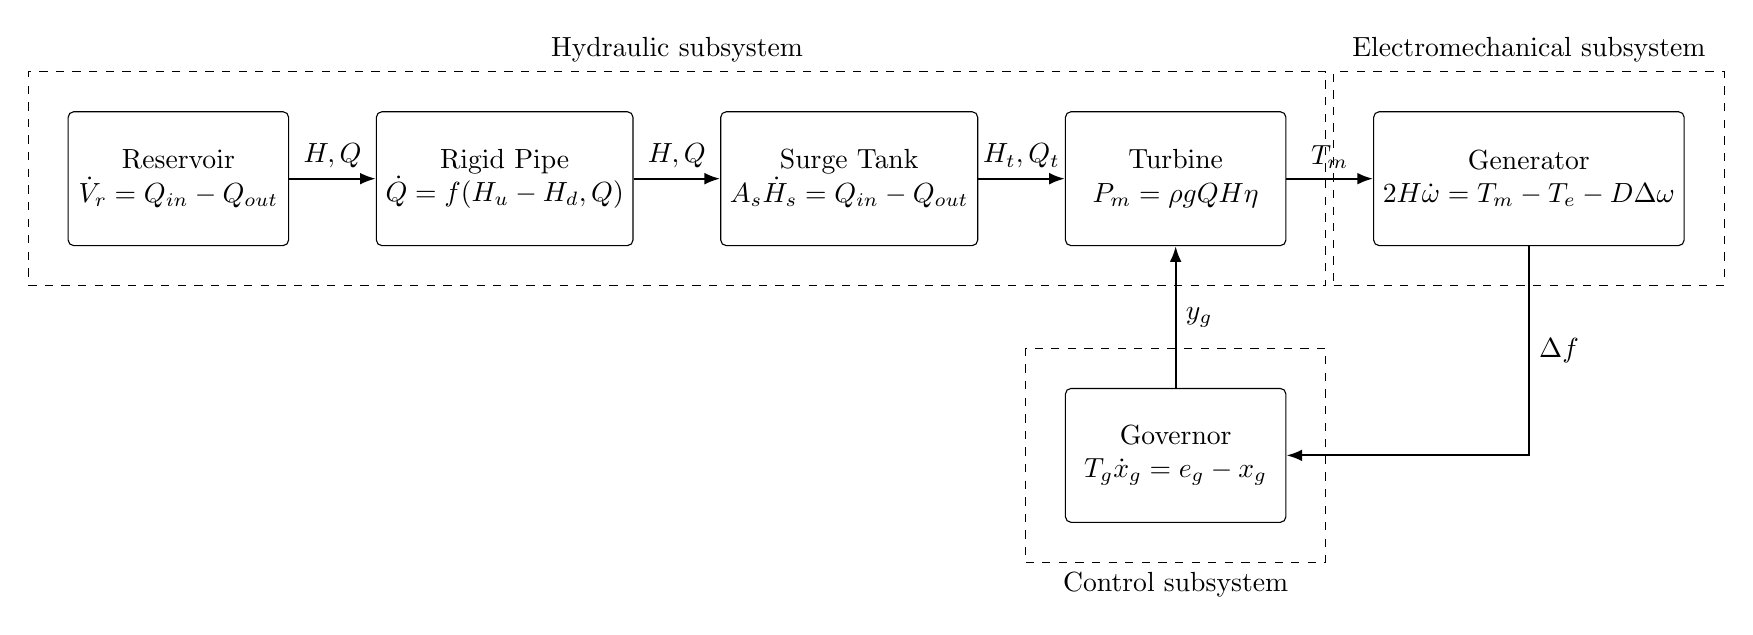
\begin{tikzpicture}[node distance=11mm]

\node[comp] (res) {Reservoir\\$\dot V_r=Q_{in}-Q_{out}$};
\node[comp,right=of res] (pipe) {Rigid Pipe\\$\dot Q=f(H_u-H_d,Q)$};
\node[comp,right=of pipe] (surge) {Surge Tank\\$A_s\dot H_s=Q_{in}-Q_{out}$};
\node[comp,right=of surge] (turb) {Turbine\\$P_m=\rho gQH\eta$};
\node[comp,right=of turb] (gen) {Generator\\$2H\dot\omega=T_m-T_e-D\Delta\omega$};

\node[comp,below=18mm of turb] (gov) {Governor\\$T_g\dot x_g=e_g-x_g$};

\draw[arr] (res) -- node[above] {$H,Q$} (pipe);
\draw[arr] (pipe) -- node[above] {$H,Q$} (surge);
\draw[arr] (surge) -- node[above] {$H_t,Q_t$} (turb);
\draw[arr] (turb) -- node[above] {$T_m$} (gen);
\draw[arr] (gov) -- node[right] {$y_g$} (turb);
\draw[arr] (gen.south) |- node[pos=0.25,right] {$\Delta f$} (gov.east);

\node[draw,dashed,fit=(res)(pipe)(surge)(turb),inner sep=5mm,label=above:{Hydraulic subsystem}] {};
\node[draw,dashed,fit=(gen),inner sep=5mm,label=above:{Electromechanical subsystem}] {};
\node[draw,dashed,fit=(gov),inner sep=5mm,label=below:{Control subsystem}] {};

\end{tikzpicture}
\end{document}
